\section{Prior update: Optimal Bayesian Kalman Filter}

\begin{frame}
    \tableofcontents[currentsection]
\end{frame}

\subsection{Basic Idea}
\begin{frame}{Basic Idea: OBKF}
    \begin{itemize}
        \item Based on the IBR Kalman Filter
        \item Utilize measured data $\mathcal{Y}_{k}=\{{\bf y}_0,...,{\bf y}_{k}\}$to obtain the posterior distribution $\pi(\theta|\mathcal{Y}_k)$
        \item Best estimation relative to $\pi(\theta|\mathcal{Y}_{k-1})$: $\argmin_{{\bf \hat x_\theta}(k)} E_\theta[E[|{\bf x_\theta}(k) - {\bf \hat x_\theta}(k)|^2]|\mathcal{Y}_{k-1}]$
    \end{itemize}
\end{frame}


\subsection{Algorithm}
\begin{frame}{Algorithm: OBKF}
\begin{itemize}
    \item OBKF is obtained just replacing ${\bf Q}$ and ${\bf R}$ in Classic Kalman Filter with $E_{\theta_1}[{\bf Q^{\theta_1}}|\mathcal{Y}_k]$ and $E_{\theta_2}[{\bf R^{\theta_2}}|\mathcal{Y}_k]$ respectively
\end{itemize}
\begin{algorithm}[H]
\caption{OBKF}
\begin{algorithmic}[1]
\REQUIRE ${\bf \hat x}^{\theta}_k$, $E_\theta[{\bf P^{x, \theta}}_{k}|\mathcal{Y}_{k-1}]$, $\mathcal{Y}_k$
\STATE $\tilde {\bf z}^{\bf \theta}_k = {\bf y}^{\bf \theta}_k - {\bf H}_k{\bf \hat x}^{\bf \theta}_k$
\STATE ${\bf K}^{\bf \Theta^*}_k = E_\theta[{\bf P^{x, \theta}}_k|\mathcal{Y}_{k-1}]{\bf H}^T_kE_\theta^{-1}[{\bf H}_k{\bf P^{x, \theta}}_k{\bf H}^T_k+{\bf R^{\theta_2}}|\mathcal{Y}_{k-1}]$
\STATE $\hat{\bf x}^{\theta}_{k+1} = {\bf \Phi}_k{\bf \hat x}^{\theta}_k+{\bf \Phi}_k{\bf K}^{\bf \Theta}_k{\bf \tilde z}^{\theta}_k$
\STATE $E_\theta[{\bf P^{x, \theta}}_{k+1}|\mathcal{Y}_k] = {\bf \Phi}_k({\bf I}-{\bf K}^{\bf \Theta^*}_k{\bf H}_k)E_\theta[{\bf P^{x, \theta}}_k|\mathcal{Y}_k]{\bf \Phi}^T_k + {\bf \Gamma}_kE_{\theta_1}[{\bf Q^{\theta_1}}|\mathcal{Y}_k]{\bf \Gamma}_k^T$
\ENSURE ${\bf \hat x}^{\theta}_{k+1}$, $E_\theta[{\bf P^{x, \theta}}_{k+1}|\mathcal{Y}_{k}]$
\end{algorithmic}
\end{algorithm}

\pause

How are the posterior expectations found: $E_{\theta_1}[{\bf Q^{\theta_1}}|\mathcal{Y}_k]$ and $E_{\theta_2}[{\bf R^{\theta_2}}|\mathcal{Y}_k]$ ?

\end{frame}

\subsection{Find Posterior Expectations}
\begin{frame}{Find Posterior Expectatoins: $E_{\theta_1}[{\bf Q^{\theta_1}}|\mathcal{Y}_k]$ and $E_{\theta_2}[{\bf R^{\theta_2}}|\mathcal{Y}_k]$}
\begin{itemize}
    \item Approximate $E_{\theta_1}[{\bf Q^{\theta_1}}|\mathcal{Y}_k]$ and $E_{\theta_2}[{\bf R^{\theta_2}}|\mathcal{Y}_k]$ using Metropolis Hastings MCMC
    \item MCMC requires the likelihood function $f(\mathcal{Y}_k|\theta)$
    \item $f(\mathcal{Y}_k|\theta)$ is calculated by sum-product algorithm\cite{Kschischang2001}
\end{itemize}
\end{frame}

\begin{frame}{Algorithm: Likelihood Function Calculation}

\begin{algorithm}[H]
\caption{Factor-Graph-Based Likelihood Function Calculation}
\begin{algorithmic}[1]
\REQUIRE $\theta$, $\mathcal{Y}_k$
\STATE ${\bf M}_0 \leftarrow E[{\bf x}_0],\; S_0 \leftarrow 1,\; {\bf \Sigma}_0 \leftarrow cov[{\bf x}_0], \; i \leftarrow 0$
\WHILE {$i \leq k-1$}
    \STATE ${\bf W}_i\leftarrow {\bf H}_i^T({\bf R}^{\theta_2})^{-1}{\bf y}_i + {\bf \Sigma}_i^{-1}{\bf M}_i$
    \STATE ${\bf \Lambda}_i^{-1}\leftarrow {\bf \Phi}_i^T({\bf \tilde Q}_i^{\theta_1})^{-1}{\bf \Phi}_i + {\bf H}_i^{T}({\bf R}^{\theta_2})^{-1}{\bf H}_i+{\bf \Sigma}_i^{-1}$
    \STATE ${\bf \Sigma}_{i+1}^{-1}\leftarrow ({\bf \tilde Q}_i^{\theta_1})^{-1} - ({\bf \tilde Q}_i^{\theta_1})^{-1}{\bf \Phi}_i{\bf \Lambda}_i{\bf \Phi}_i^T({\bf \tilde Q}_i^{\theta_1})^{-1}$
    \STATE ${\bf M}_{i+1}\leftarrow {\bf \Sigma}_{i+1}({\bf \tilde Q}_i^{\theta_1})^{-1}{\bf \Phi_i}{\bf \Lambda}_i({\bf H}_i^T({\bf R}^{\theta_2})^{-1}{\bf y}_i+{\bf \Sigma}_i^{-1}{\bf M}_i)$
    \STATE $S_{i+1} \leftarrow \text{using Eq.(29) in the paper}$
    \STATE $i \leftarrow i+1$
\ENDWHILE
\STATE ${\bf \Delta}_k^{-1}\leftarrow {\bf H}_k^T({\bf R}^{\theta_2})^{-1}{\bf H}_k + {\bf \Sigma}_k^{-1}$
\STATE ${\bf G}_k \leftarrow {\bf \Delta}_k({\bf H}_k^T({\bf R}^{\theta_2})^{-1}{\bf y}_k + {\bf \Sigma}_k^{-1}{\bf M}_k)$
\STATE $f(\mathcal{Y}_k|\theta) \leftarrow \text{using Eq.(34) in the paper}$
\ENSURE $f(\mathcal{Y}_k|\theta)$
\end{algorithmic}
\end{algorithm}
\end{frame}

\subsection{Performance}

\begin{frame}{Performance: Accuracy}
% Good image will inserted here
% Bigger figure
\pnote{
    * figureはtheta1=1, theta2=knownの時のlocalizationについてのシミュレーション結果を示している。
    * figureは各カルマンフィルタの精度を示している。縦軸が精度と同じだと思ってくれて構わない。黒線はtheta1=1を使用したクラシックカルマンフィルタであり、これ以上の精度は出すことは出来ない。図より、OBKFは他の手法と比較して最も早く最適なカルマンフィルタにconvergeしていることがわかる。
}
\begin{figure}[H]
    \begin{center}
    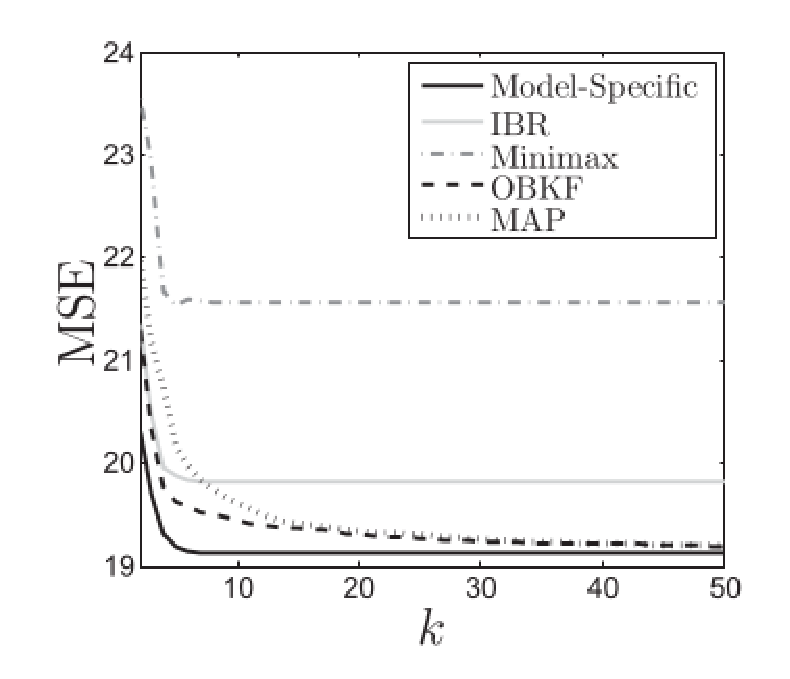
\includegraphics[width=7cm]{img/OBKF_r1.eps}
    \caption{Performance analysis for specific $\theta_1 = 1$ and known $\theta_2$  \protect\linebreak OBKF achieves the lowest MSE (cited from \cite{Dehghannasiri2018})}
    \label{fig:r_1}
    \end{center}
\end{figure}
\end{frame}

\begin{frame}{Performance: Data Efficiency}
    \pnote{
    * figureはthetaがunknownであるときに高いMSEを達成するのに必要なstep数kを示している。
    }
\begin{figure}[H]
    \begin{center}
    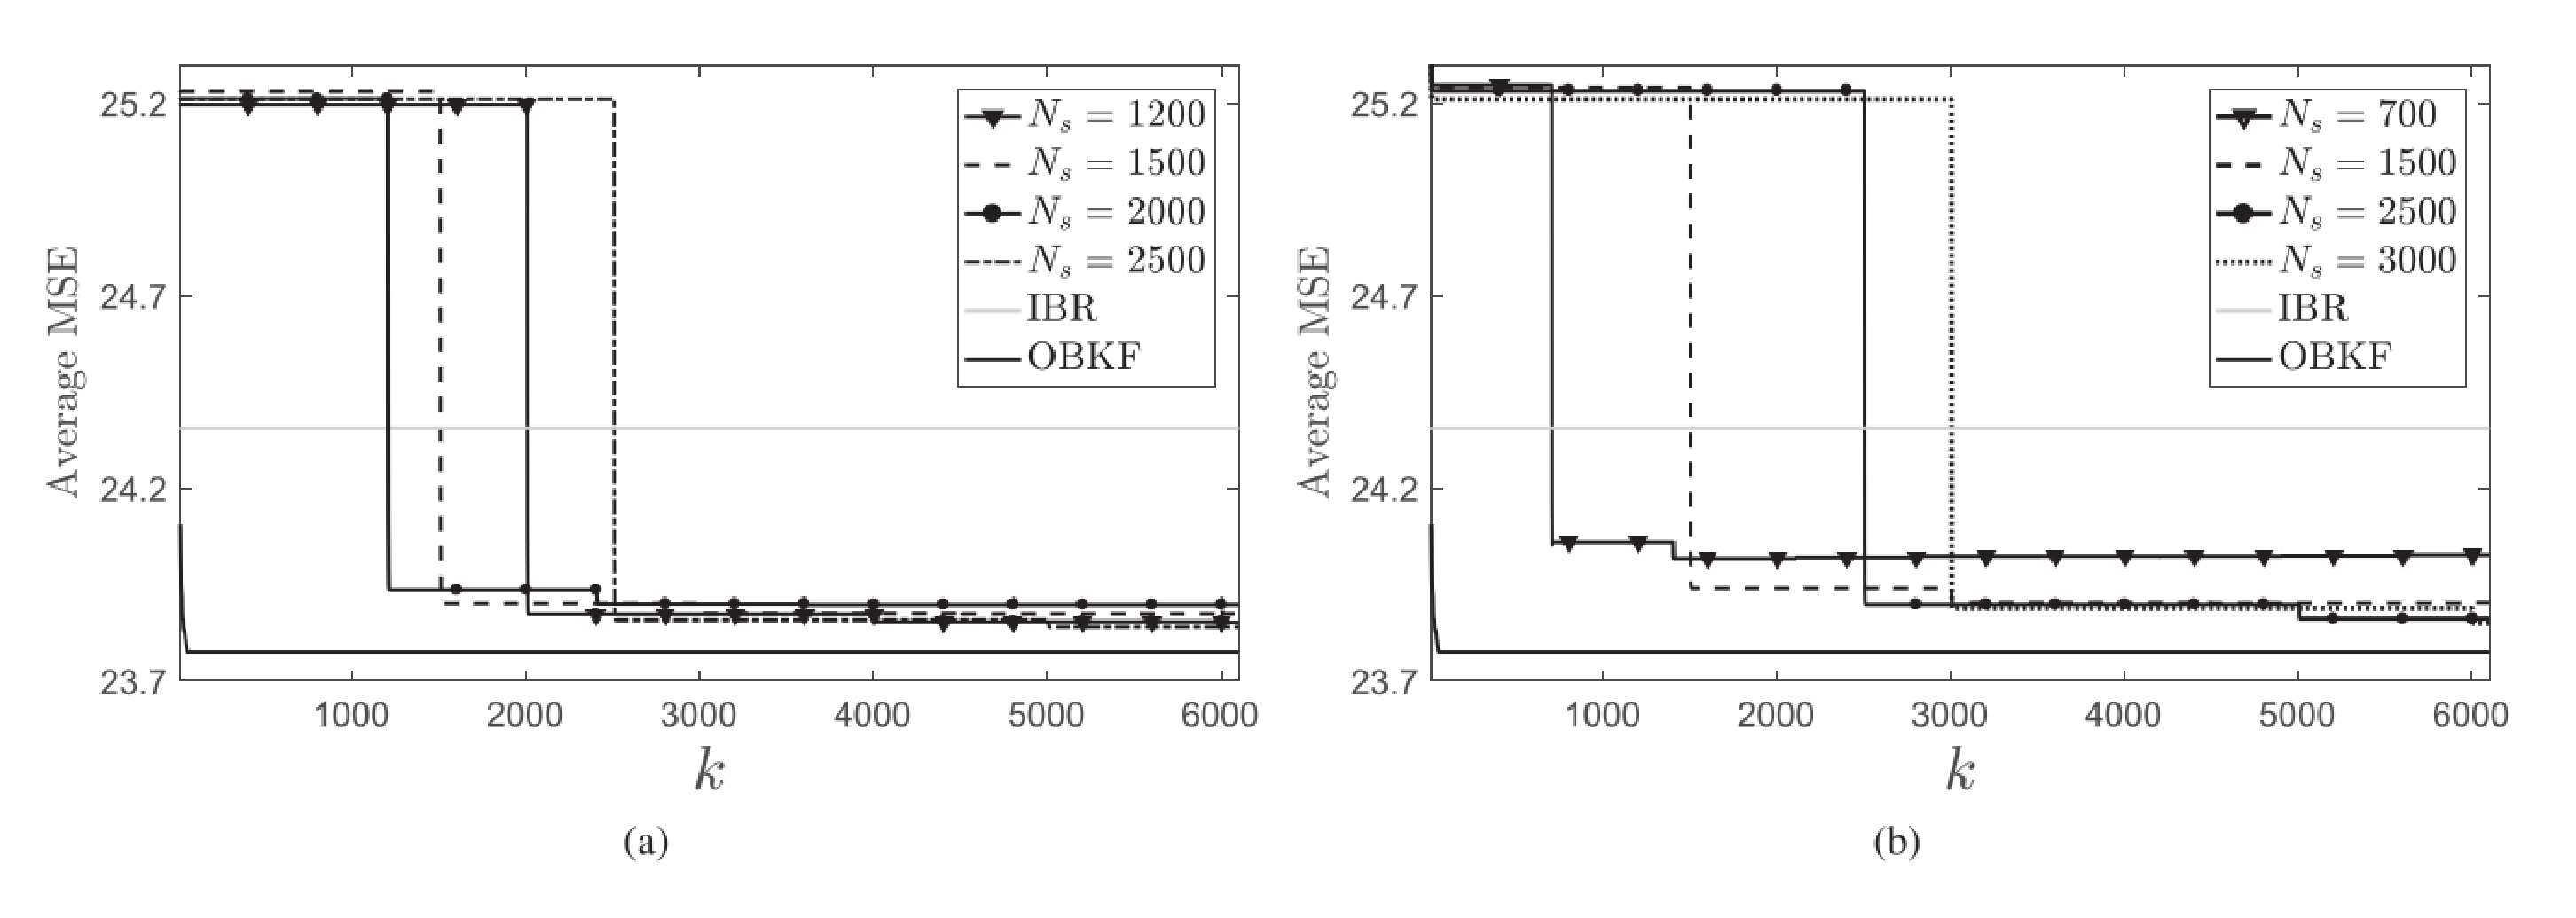
\includegraphics[width=9cm]{img/cmp_adaptive.eps}
    \caption{Unknown $\theta_1$ and comparison with an adaptive Kalman Filter (cited from \cite{Dehghannasiri2018})}
    \label{fig:cmp_adaptive}
    \end{center}
\end{figure}

\end{frame}


\subsection{Problems and Future Works}
\begin{frame}{Problems and Future Works}
\begin{itemize}
    \item If the prior distribution doesn't include the true value, the estimation won't converge
    \item Factor-graph and MCMC are computationally expensive. Finding an efficient approach is a future work.
\end{itemize}
\end{frame}